\chapter{Simulation}
\label{sec:simulation}
\section{RAT}
\begin{figure}[htbp]
\centering
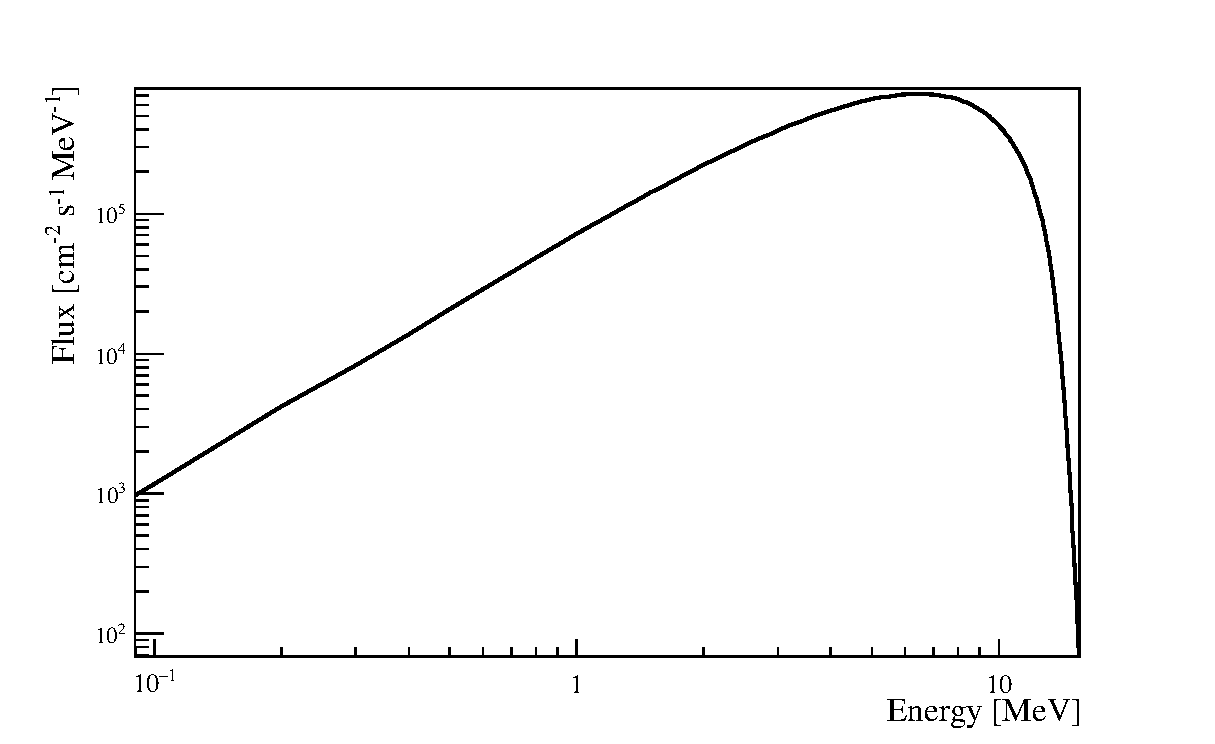
\includegraphics[width=0.75\textwidth]{b8_flux}
\caption[Expected $\ce{^{8}B}$ Flux]{The $\ce{^{8}B}$ neutrino flux
normalized to the solar reaction rate predicted by BS05-0P~\citep{bs_ssm}}
\label{fig:b8_flux}
\end{figure}

RAT, a Monte Carlo simulation of particle interactions in the detector is used
for predicting detector observables for solar neutrino and background events.
RAT is a Geant4-based~\citep{geant4} simulation that
contains a detector and DAQ simulation in addition to simulation of particle
interactions and photon propagation.

The first step in the Monte Carlo event simulation process is to generate
event vertex information, including the interaction location, and the neutrino
and recoil electron energy and direction.
The distribution for the $\ce{^{8}B}$ neutrino energy from Winters~\textit{et.\ al.}~\citep{winterspectrum}
was used, normalized to a nominal flux of
$\Phi_{\nu_{\mathrm{e}}} = 9.67\times10^{9}\mathrm{cm}^{-2}\mathrm{s}^{-1}$
and
$\Phi_{\nu_{\mathrm{\mu}}} = 5.46\times10^{10}\mathrm{cm}^{-2}\mathrm{s}^{-1}$.
These values are the full BS05OP~\cite{bs_ssm} $\ce{^{8}B}$ flux scaled by a factor
of $1700$ for the $\nu_{\mathrm{e}}$ and a factor of $9600$ for the $\nu_{\mathrm{\mu}}$.
The overall flux normalization is arbitrary in this analysis, but the enhanced rate
ensures that the statistical fluctuations observed in the MC datasets are
negligible compared to the detected dataset.

\begin{figure}[htbp]
  \centering
  \begin{subfigure}[b]{0.48\textwidth}
    \centering
  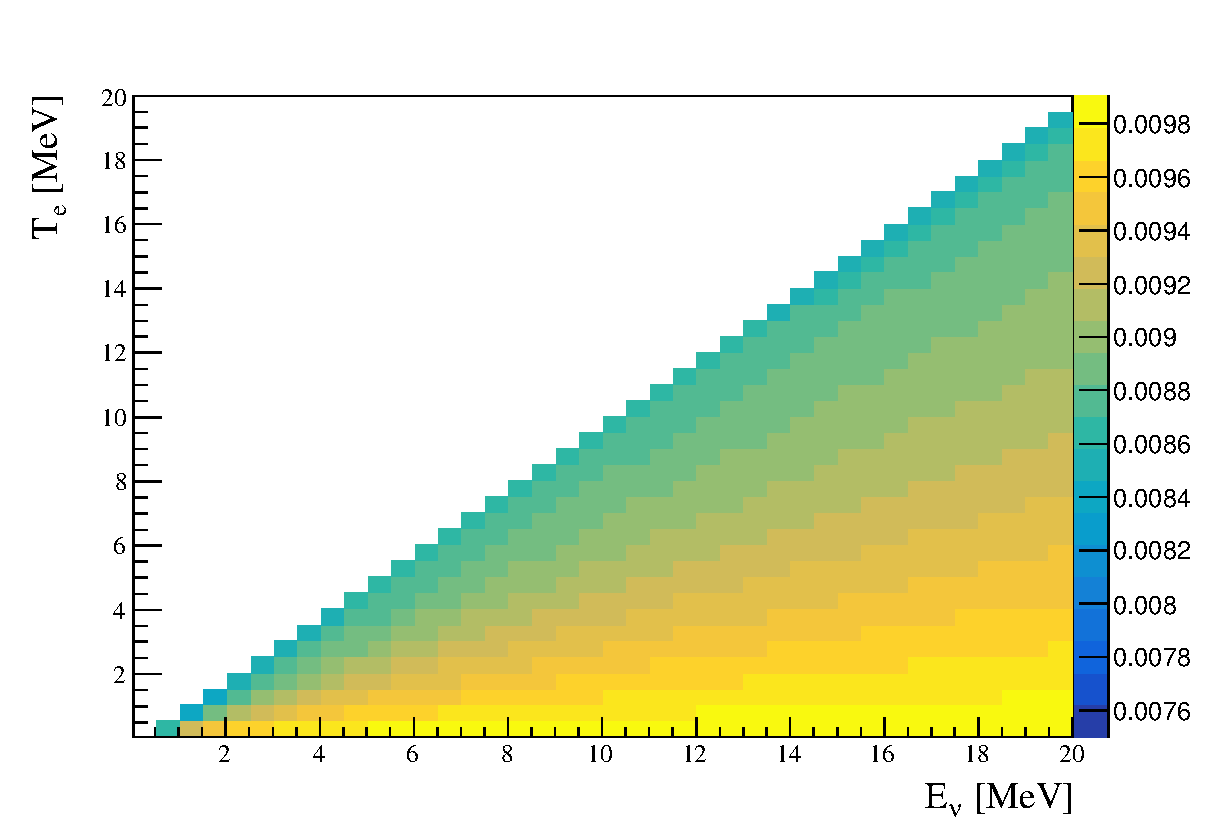
\includegraphics[width=\textwidth]{diff_xsec_nue}
    \caption[$\nu_{e}$ Differential Cross Section]{}
    \label{fig:diff_xsec_nue}
  \end{subfigure}
  \hfill
  \begin{subfigure}[b]{0.48\textwidth}
    \centering
  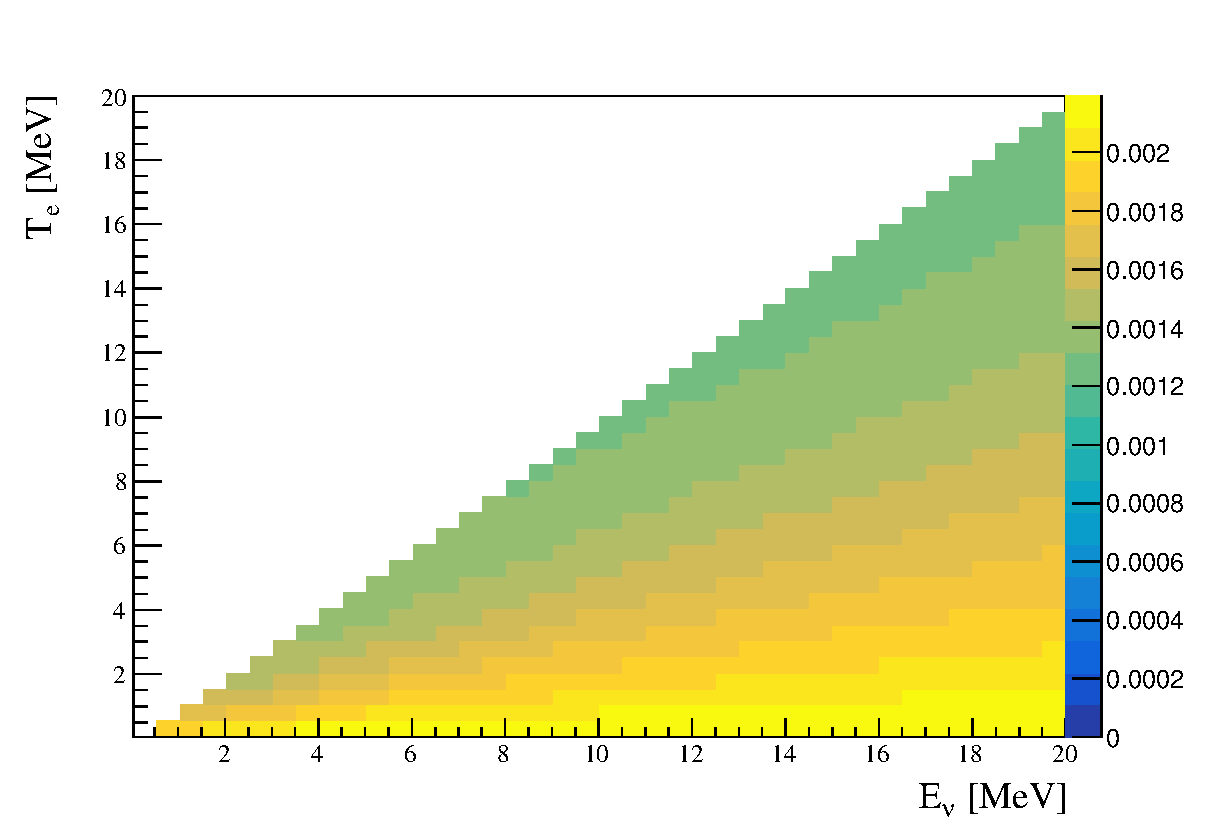
\includegraphics[width=\textwidth]{diff_xsec_numu}
    \caption[$\nu_{\mu}$ Differential Cross Section]{}
    \label{fig:diff_xsec_numu}
  \end{subfigure}
    \caption[ES Differential Cross Section]{The differential cross section for $\nu_{e}$ electron
    elastic scattering (a) and $\nu_{\mu\mathrm{,}\tau}$ (b) as used by
    RAT. Units for Z-axis is $10^{-42} \mathrm{cm}^{-2} \mathrm{MeV}^{-2}$.}
    \label{fig:diff_xsec}
\end{figure}

The rate of solar neutrino interactions for a given flux follows from the cross-section for
interaction. The only interaction relevant for this analysis is the
neutrino-electron elastic scattering interaction, the cross-section of which
is discussed in Sec.~\ref{sec:esxsec}.
The model used for event generation in RAT includes radiative corrections as
described in Bahcall~\textit{et. al}~\citep{escrosssec}.
The differential cross-section as a function of $E_{\nu}$ is shown in Fig.~\ref{fig:diff_xsec}.

\begin{figure}[htbp]
  \centering
  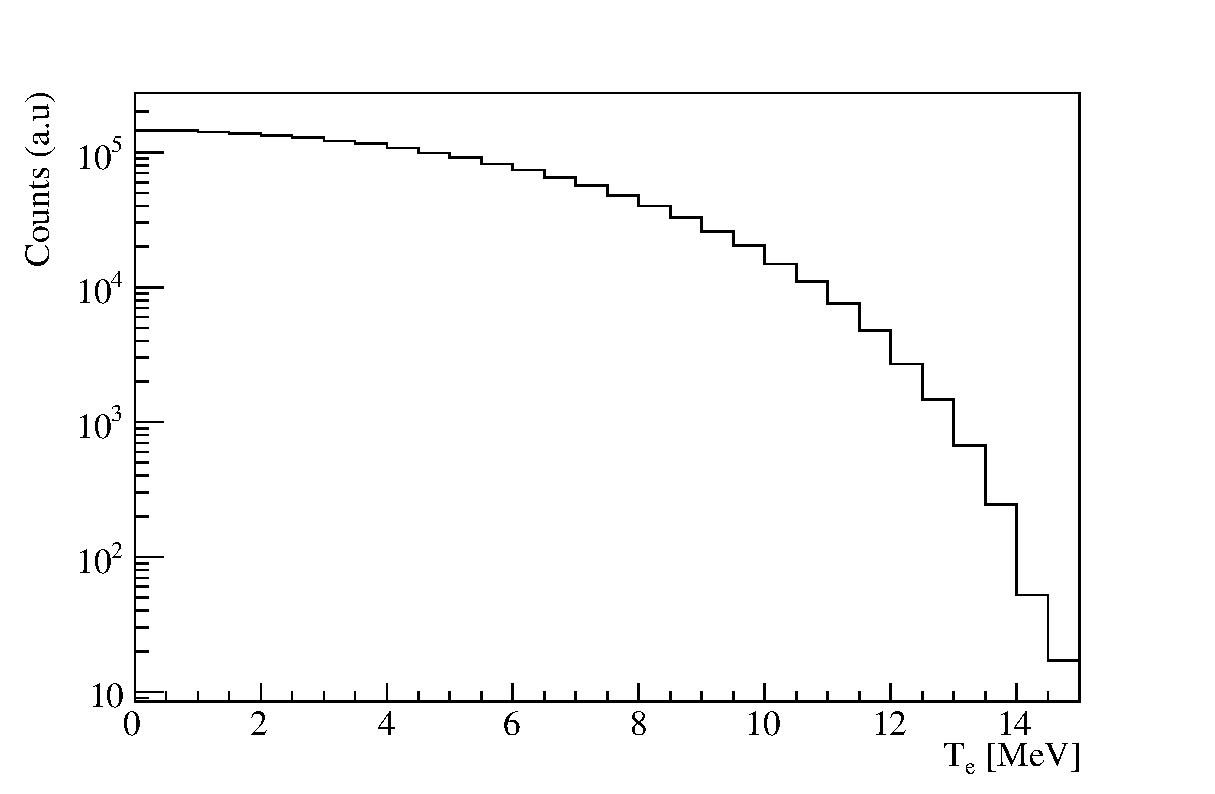
\includegraphics[width=\textwidth]{solar_nu_recoil_spectrum}
  \caption[Solar Recoil Electron Spectrum]{
      The distribution of electron recoil energies from $\ce{^{8}B}$ solar neutrino
      interactions, as simulated by RAT\@.}
    \label{fig:recoil_spectrum}
\end{figure}

Convolving the differential cross section with $\ce{^{8}B}$ neutrino flux
spectrum provides the expected event rate as a function of$T_{\mathrm{e}}$. 
RAT performs this convolution through Monte Carlo sampling of the neutrino
and cross-section PDFs.
The results of the MC sampling are show in Figure~\ref{fig:recoil_spectrum}.

Simulated recoil electrons are distributed uniformly throughout the SNO+ AV volume, with
the $\theta_{sun}$ given by,
\begin{equation}
  \cos\theta_{sun} = \sqrt{\dfrac{T_{\mathrm{e}}(m_{\mathrm{e}}+E_{\nu})^{2}}{2m_{e}E_{\nu}^{2} + E_{\nu}^{2}T_{\mathrm{e}}}}\text{.}
  \label{eqn:costheta_te}
\end{equation}
This equation assumes that the direction of the neutrino is directly from the center of sun.
Averaged over many events that is a safe assumption; the additional angular uncertainty
introduced by considering the radial neutrino production distribution is negligible.

Once the simulated position, direction, and energy of the recoil electron are determined  the
electron interactions and  photon production and propagation in the detector are simulated
by Geant4~\citep{geant4}.
The goal of this simulation is to transform the kinematics of the event to
a collection of PMT hits in the simulated detector.
In the simulation, once a photon interacts with a PMT photo-cathode, a check is performed
to simulate the detection efficiency for that photon, which includes the photo-cathode quantum efficiency and
PMT collection efficiency.
These efficiencies are determined from both \textit{ex-situ} PMT measurements
and~\textit{in-situ} calibration measurement.
The collection efficiencies are
taken to be uniform across the detector. %TODO Citation?
If the photon passes that check a PMT signal is created in the DAQ simulation.
Once all the photons in an event have been simulated and have either exited the detector,
been detected, or been absorbed, the DAQ simulation is run on the detected photon signals.

The goal of the DAQ simulation is to transform simulated PMT hits to detector observables,
\textit{e.g.} QHS, hit times, trigger information etc.
The DAQ simulation accomplishes this by replicating the trigger system of the real SNO+ detector.
It starts by creating waveforms for every simulated PMT signal, the size
of the PMT signal is drawn from the charge spectrum for each PMT as determined
by the PCA calibration.
Electronics noise is added to each simulated waveform, then each waveform is compared to a discriminator
threshold, the value for which is matched to detector settings.
For signals that pass the discriminator threshold a PMT hit is created
and N100, N20, ESUMH and ESUML trigger signals are produced.
The waveforms for the trigger signals are simulated with electronic noise and dropout, both
of which match detector measurements.
The trigger signals are then summed detector wide and compared to ``MTCA+'' thresholds.
If any of the threshold crossing signals are included in the simulated trigger mask
each hit's  QHS, QHL, QLX, and threshold crossing time, are calculated from the original PMT waveform.
The trigger waveforms are also digitized in a simulated 12-bit digitizer with sampling rate matched
to that of the CAEN v1720 digitizer.

\begin{figure}[htbp]
  \centering
  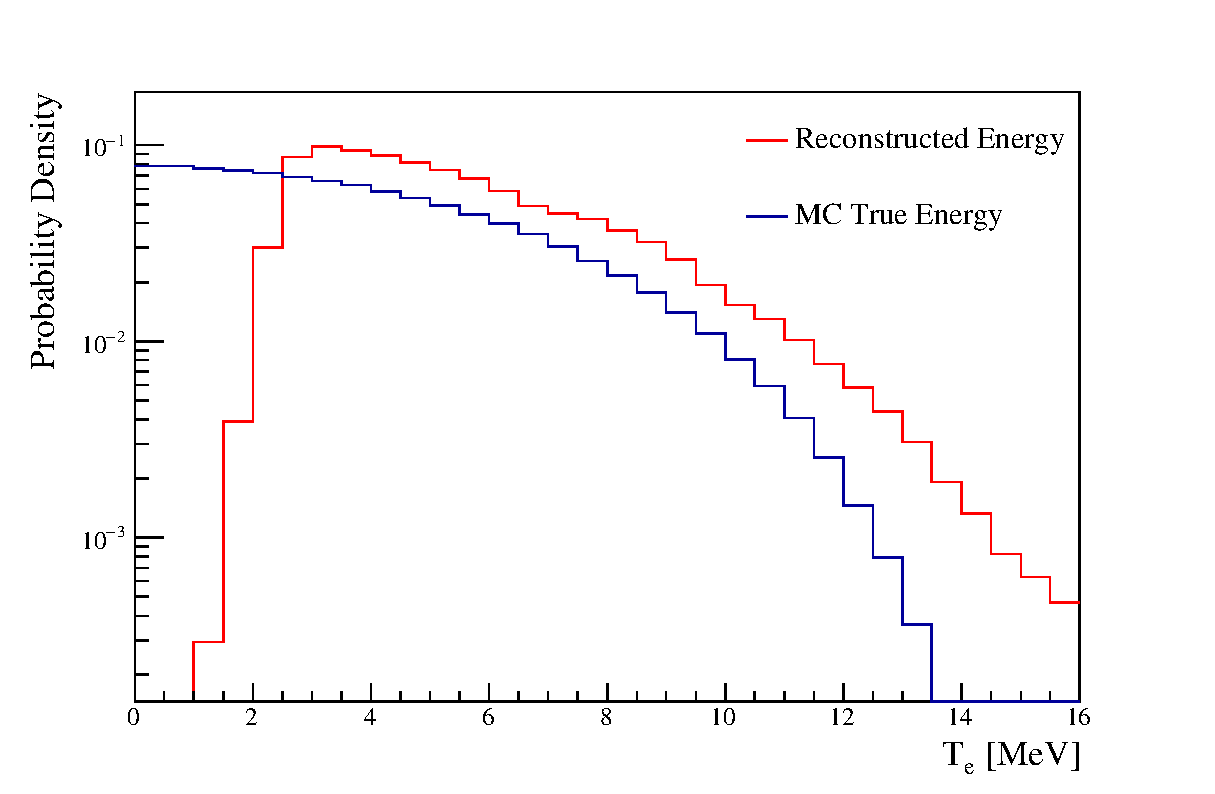
\includegraphics[width=0.7\textwidth]{energy_comparison}
  \caption[Reconstructed Energy Vs True Energy]{ The distributions of recoil
  electron truth energy (black) and reconstructed energy (red) for simulated
  $\ce{^{8}B}$ $\nu_{e}$ elastic-scatter events. Both histograms are normalized to $1.0$.} %TODO normalize them the number simulated instead
  \label{fig:energy_comparison}
\end{figure}

The result of the DAQ simulation is a dataset that can be used in exactly the same way the
detector data can be used.
Reconstruction is performed on the simulated detector observables 
 and the reconstructed quantities can be compared
to the corresponding MC truth values to assess expected detector performance.
The comparison between true energy and reconstructed energy is shown in
Fig.~\ref{fig:energy_comparison} for the simulated $\ce{^{8}B}$ $\nu_{e}$
dataset.
The probability of an event having a reconstructed energy below approximately 3\,MeV
is small because events with low energy will often not trigger the detector, or
fail to reconstruct at all.
Additionally to prevent the reconstruction process from being too computationally expensive
only 10\% of events with fewer than 15 PMT hits are reconstructed because
those events are generally not useful for analysis.

RAT is used to generate two MC datasets, a solar $\nu_{e}$ dataset
and a solar $\nu_{\mu}$ dataset.
No $\nu_{\tau}$ dataset is generated because the SNO+ detector has
no way to discriminate between $\nu_{\mu}$ and $\nu_{\tau}$ elastic scatters.
So the $\nu_{\mu}$ dataset can be considered to represent both the $\nu_{\mu}$
and the $\nu_{\tau}$ components of the solar neutrino flux.
The simulated solar neutrino datasets restrict interactions to the AV volume,
further datasets were generated that simulate interactions exclusively in the
volume between the AV and PSUP\@.
These external datasets contribute negligibly to the final dataset after all
analysis cuts are performed, and so they are in general not considered.

Also generated are a number of datasets for the expected backgrounds from
radioactive isotopes in various detector components.
These datasets are not directly used in this analysis, they were used however
for assessing the effectiveness of the analysis cuts that are used.

This analysis uses what is referred to as ``run-by-run'' simulation.
This means every detector data run used in the analysis has a simulated run that uses
the detector and electronic calibration settings from the run as input to the DAQ simulation, and simulates
a length of time and time of day equal to the detector run.
The purpose of this is to remove the possibility that changes in detector settings
or circumstances will bias any result.
This method is not perfect, there exists features of the real detector
that are not simulated.
For example, it's known that human activity around the DAQ electronics can generate
noise on the front end, this sort of noise source can be difficult to directly observe
in the detector data and cannot be simulated.
For this reason detector runs that have difficult to simulate conditions
are typically not included in the analysis, this is discussed further
in Sec.~\ref{sec:data_selection}.

\section{Survival Probability Simulation}
\label{sec:survival_prob}
\begin{figure}[htbp]
\centering
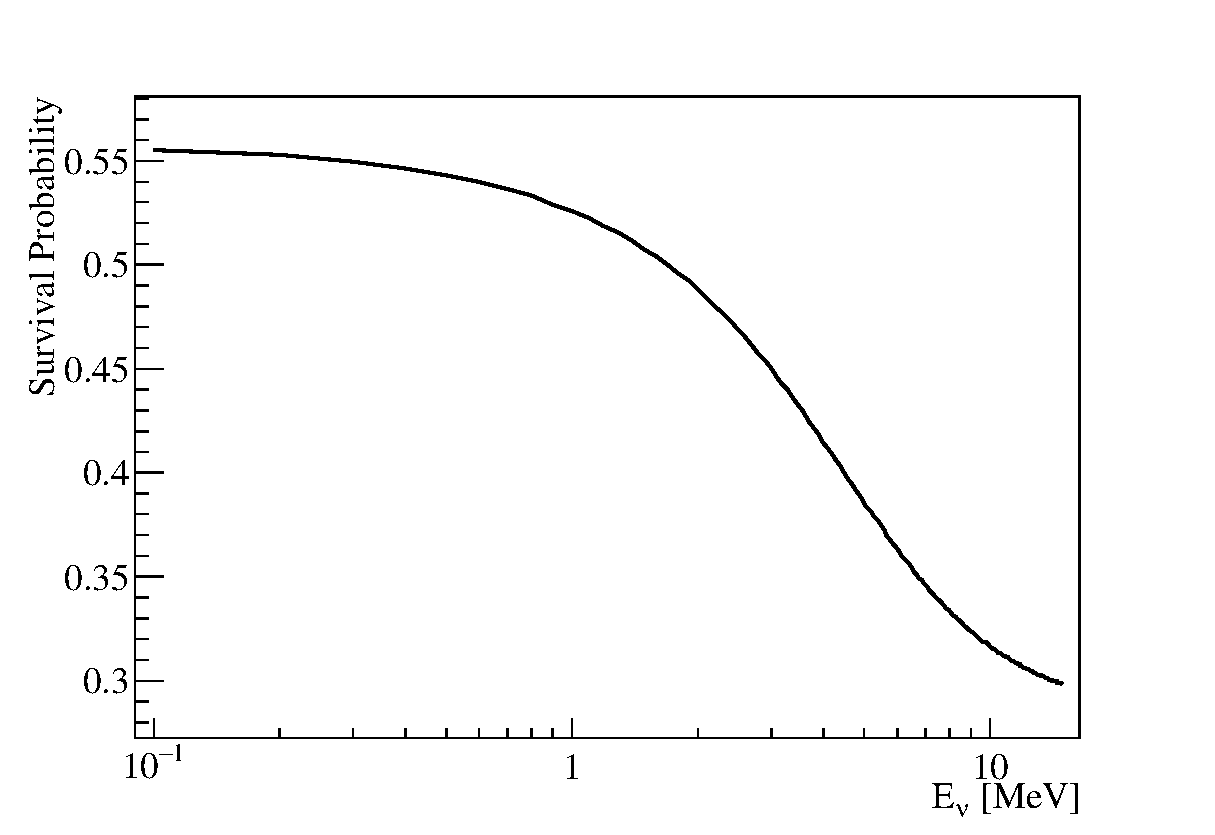
\includegraphics[width=0.75\textwidth]{pee_example}
\caption[$\ce{^{8}B}$ Solar Neutrino Survival Probability]{
Survival probability for $\ce{^{8}B}$ solar neutrinos for mixing parameters
given in table 1 of Capozzi~\textit{et.\ al.}~\citep{pdg_globalfit}.
}
\label{fig:example_survival_prob}
\end{figure}

The neutrino survival probability is simulated outside of RAT\@.
The MC $\nu_{\mathrm{e}}$ and $\nu_{\mathrm{\mu}}$ datasets are combined
as one of the last stages of this analysis to ensure that MC data
does not need to be regenerated for any change in the simulated survival probability.

The survival probability is calculated using a three-flavor adiabatic approximation.
The implementation used is the Physics interpretation Sun-Earth Large Mixing Angle Adiabatic Approximation
(PSelmaa) used in SNO~\citep{nuno_thesis, sno_combined}.
The survival probability calculation use the GS98~\citep{gs98} solar abundances
and the BS05OP radial production distributions and solar density profile~\citep{bs_ssm}.
Figure~\ref{fig:example_survival_prob} shows an example survival probability, using the best fit mixing parameters
from a global fit to neutrino oscillation data~\citep{pdg_globalfit}.
The uncertainties on those values are also considered as will be discussed in
Sec~\ref{sec:systematics}.
